\chapter{แผนภาพการออกแบบระบบ}

ในขั้นตอนทำโครงงาน เป็นห่วง เริ่มจากการออกแบบก่อนนำไปสร้างเป็นระบบจริง เนื้อหาในภาคผนวกนี้ประกอบด้วยขั้นตอนการออกแบบการทำงานของฟังก์ชันต่าง ๆ รวมถึงหน้าตาของระบบ ที่เกี่ยวข้องกับโครงงาน 
โดยเนื้อหาจะแบ่งออกเป็นสองส่วนหลัก ๆ คือ 
การออกแบบวิธีการทำงานของระบบซึ่งออกแบบโดยใช้แอปพลิเคชัน Goodnotes และการออกแบบหน้าตาของระบบซึ่งออกแบบโดยใช้โปรแกรม Adobe XD ดังนี้
\begin{figure}
  \begin{center}
    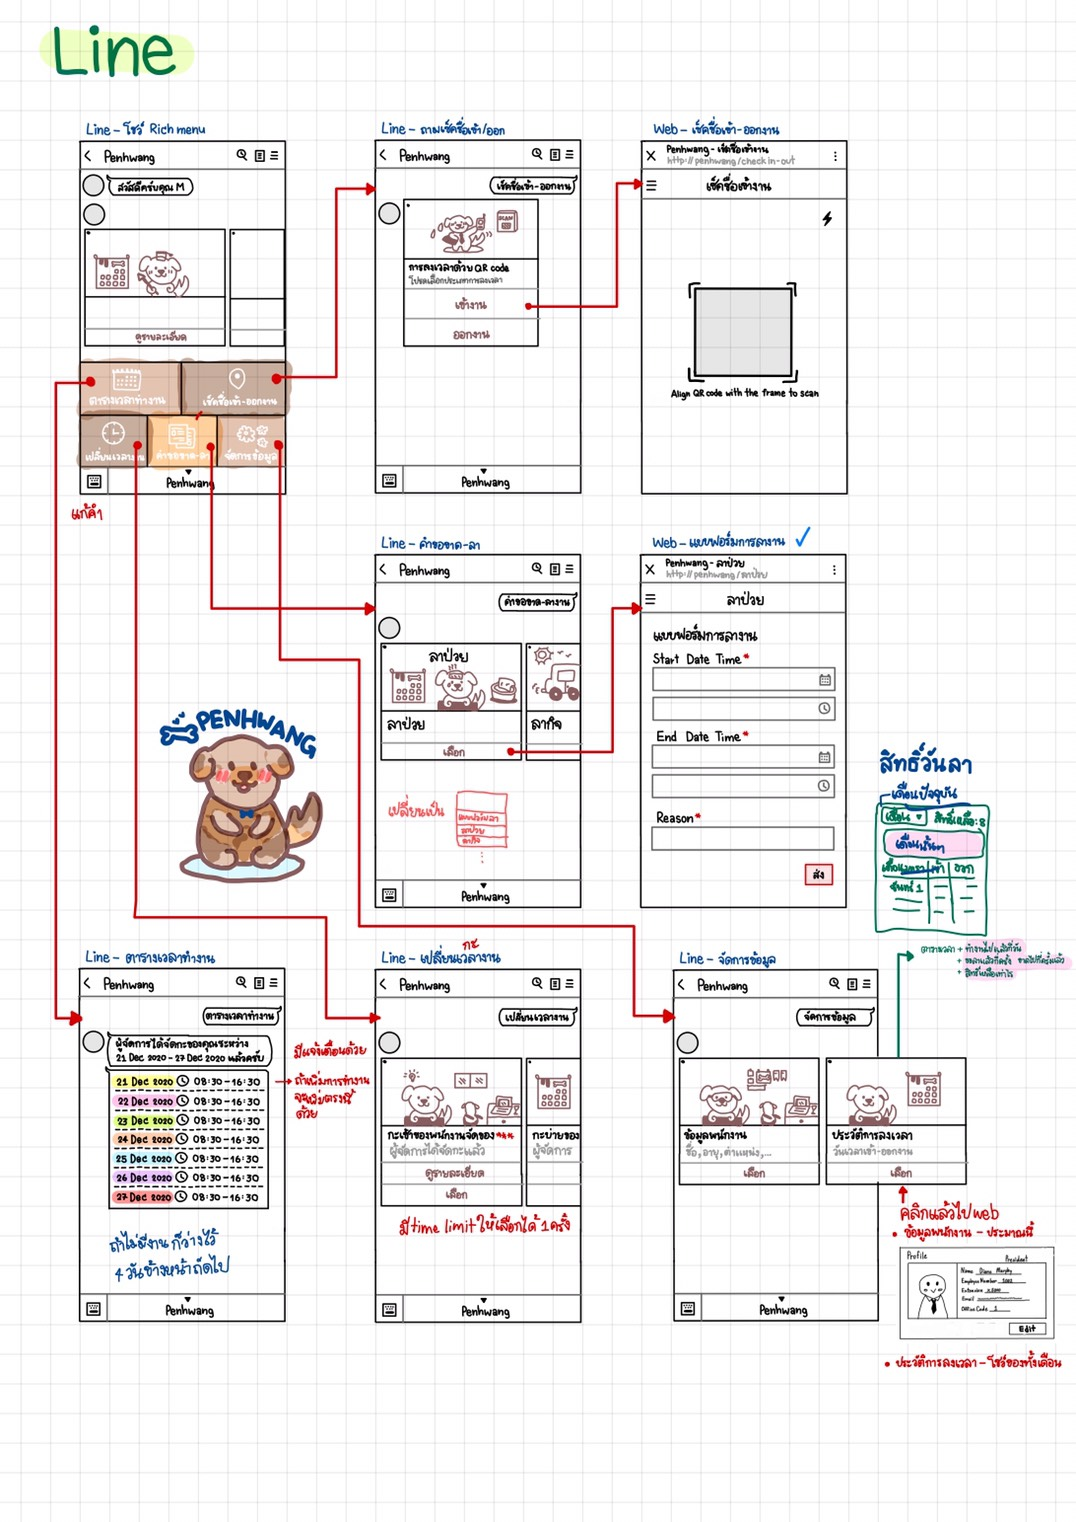
\includegraphics[width=\linewidth]{./images/design1.jpg}
  \end{center}
  \caption[รูปแสดงภาพร่างของ chatbot]{รูปแสดงภาพร่างของ chatbot} 
\end{figure}

\begin{figure}
  \begin{center}
    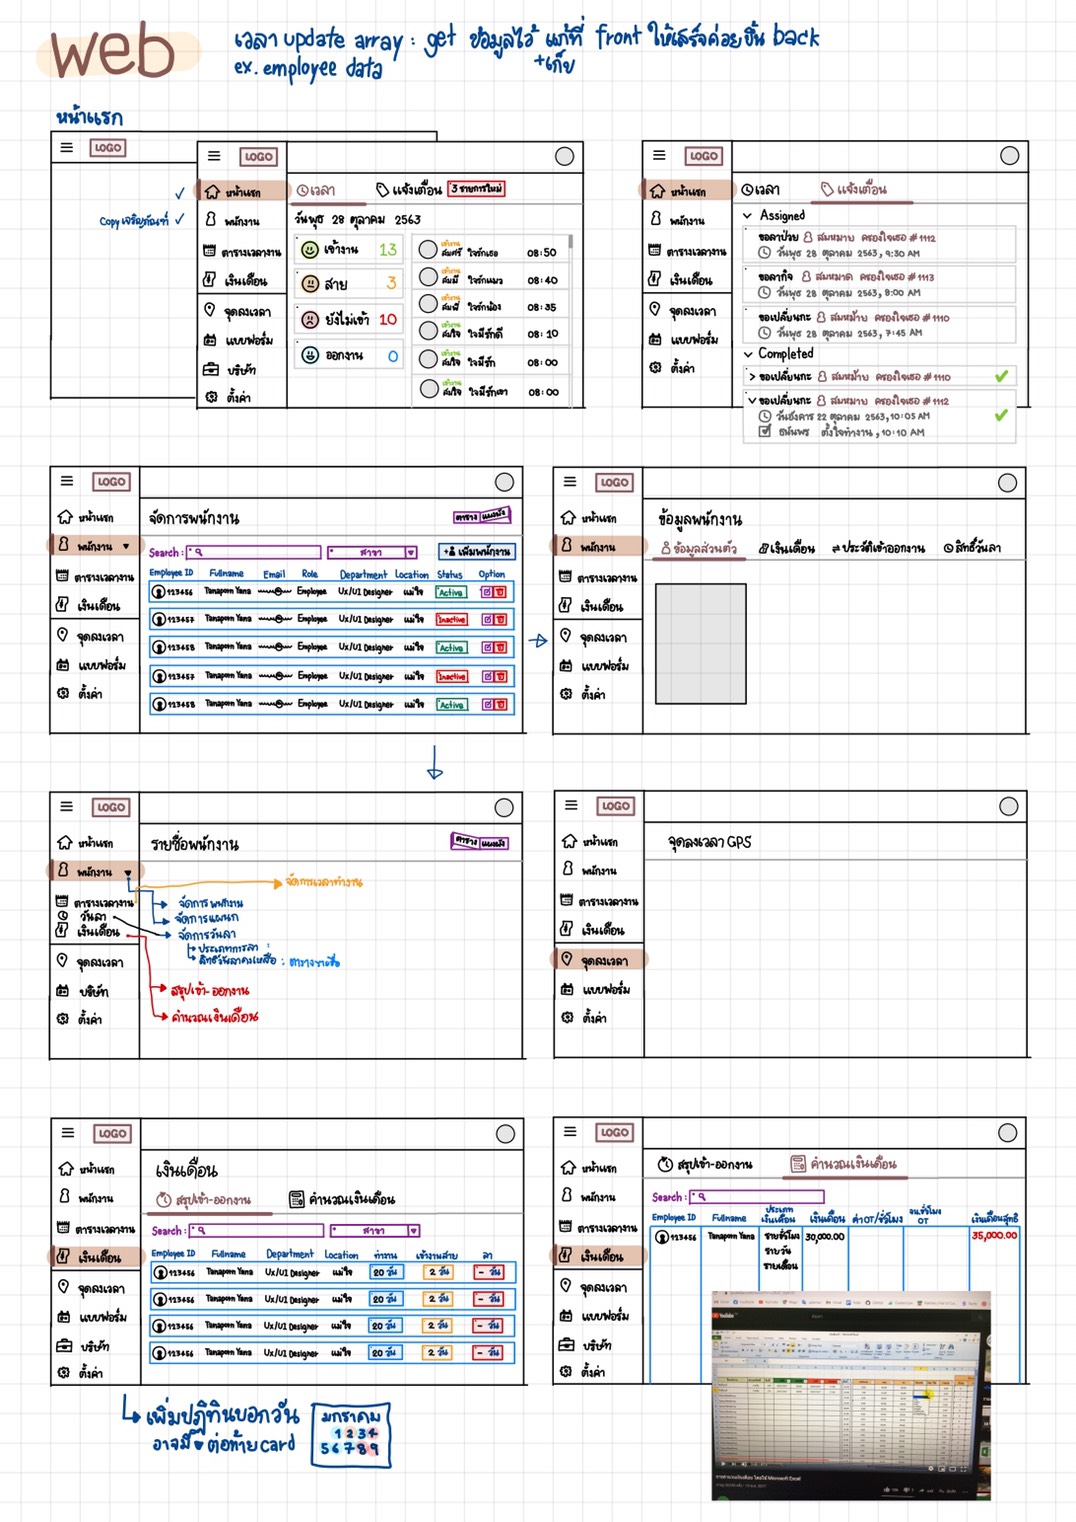
\includegraphics[width=14cm,keepaspectratio]{./images/design3.jpg}
  \end{center}
  \caption[รูปแสดงภาพร่างของเว็บแอปพลิเคชัน]{รูปแสดงภาพร่างของเว็บแอปพลิเคชัน} 
  
\end{figure}

\begin{figure}
  \begin{center}
    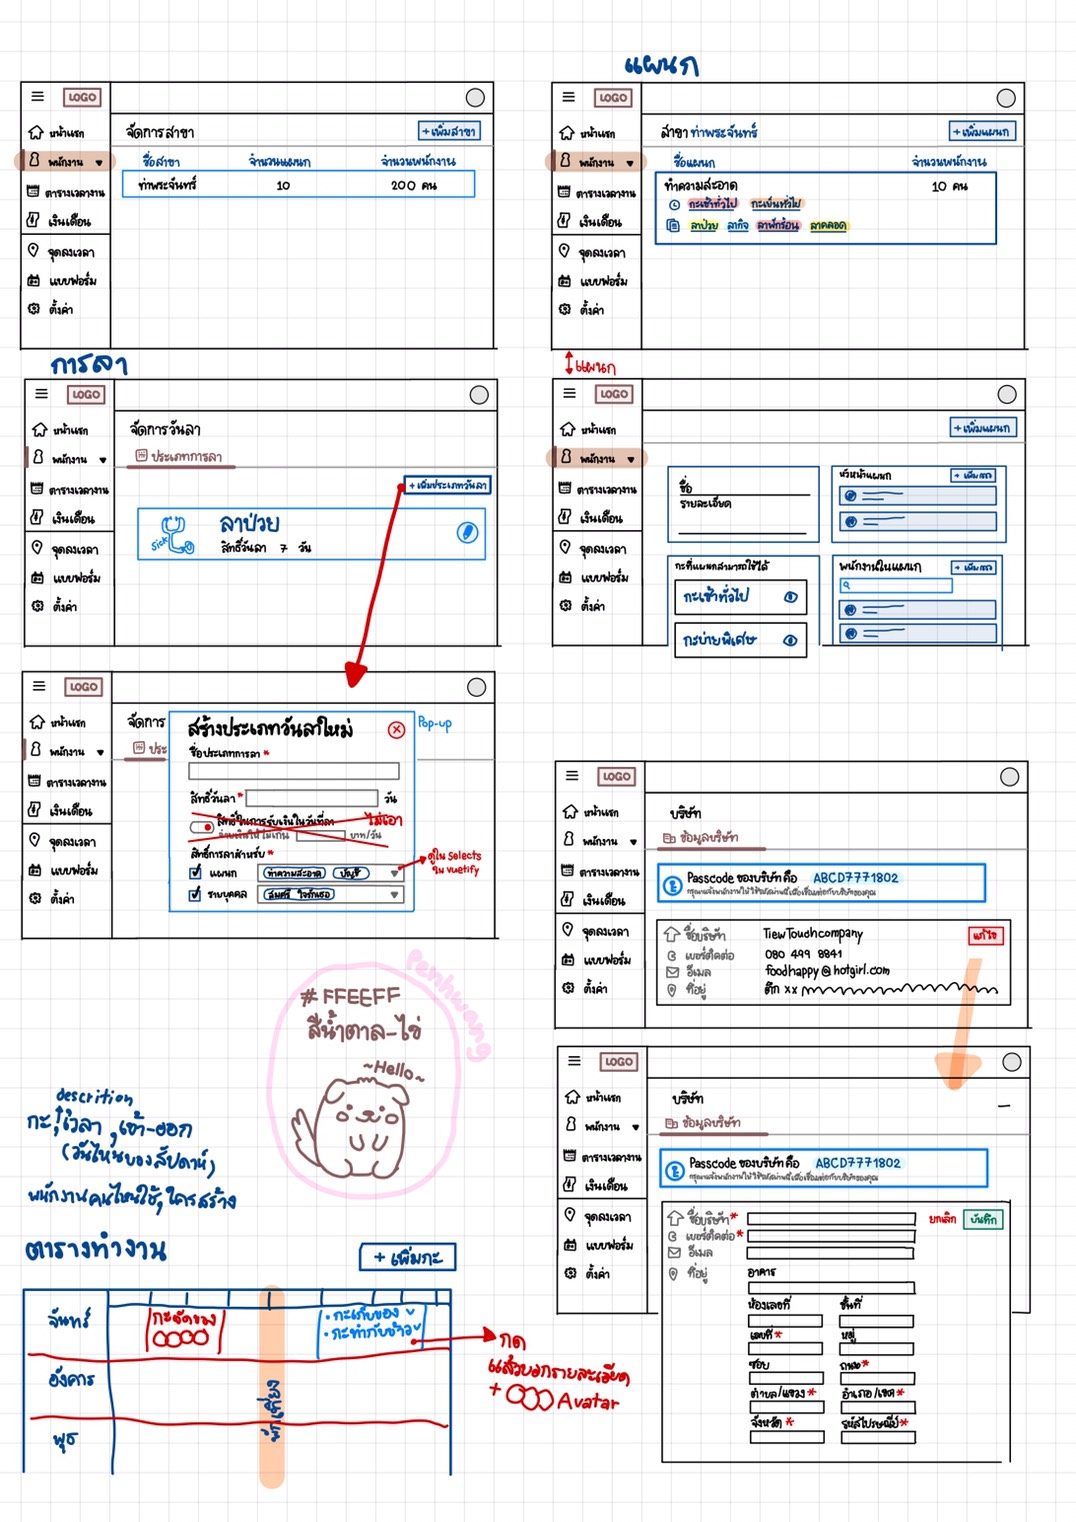
\includegraphics[width=14cm,keepaspectratio]{./images/design4.jpg}
  \end{center}
  \caption[รูปแสดงภาพร่างของเว็บแอปพลิเคชัน2]{รูปแสดงภาพร่างของเว็บแอปพลิเคชัน2} 
  
\end{figure}

\begin{figure}
  \begin{center}
    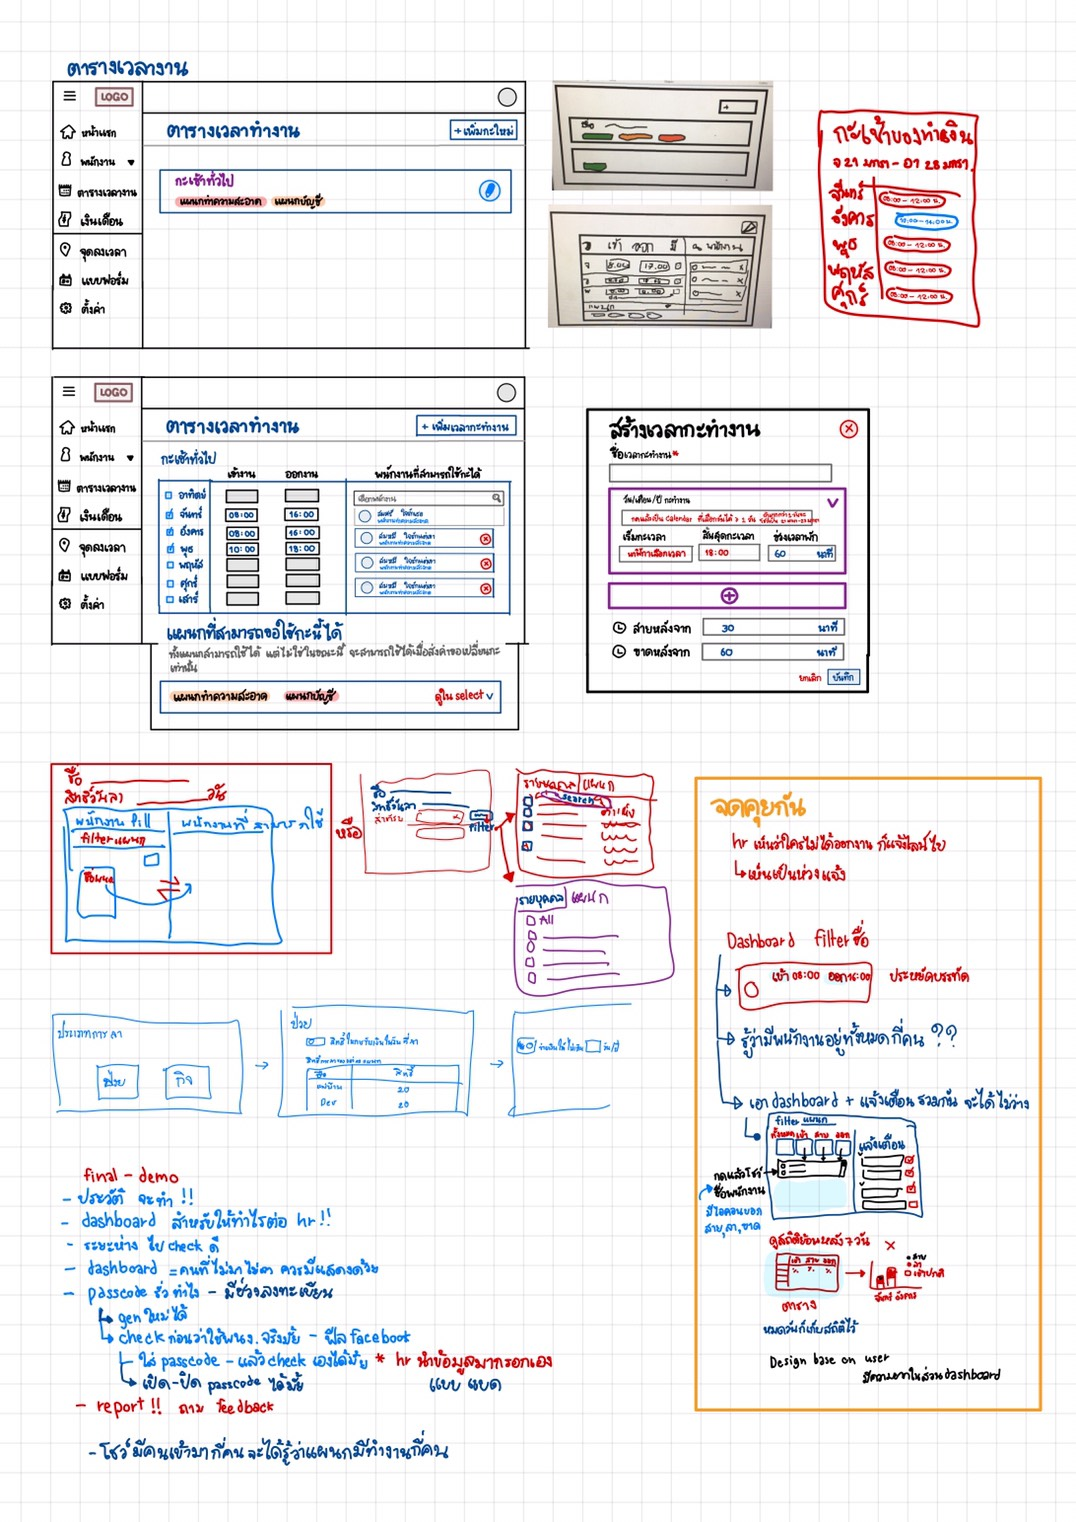
\includegraphics[width=14cm,keepaspectratio]{./images/design5.jpg}
  \end{center}
  \caption[รูปแสดงภาพร่างของเว็บแอปพลิเคชัน3]{รูปแสดงภาพร่างของเว็บแอปพลิเคชัน3} 
  
\end{figure}

\begin{figure}
  \begin{center}
    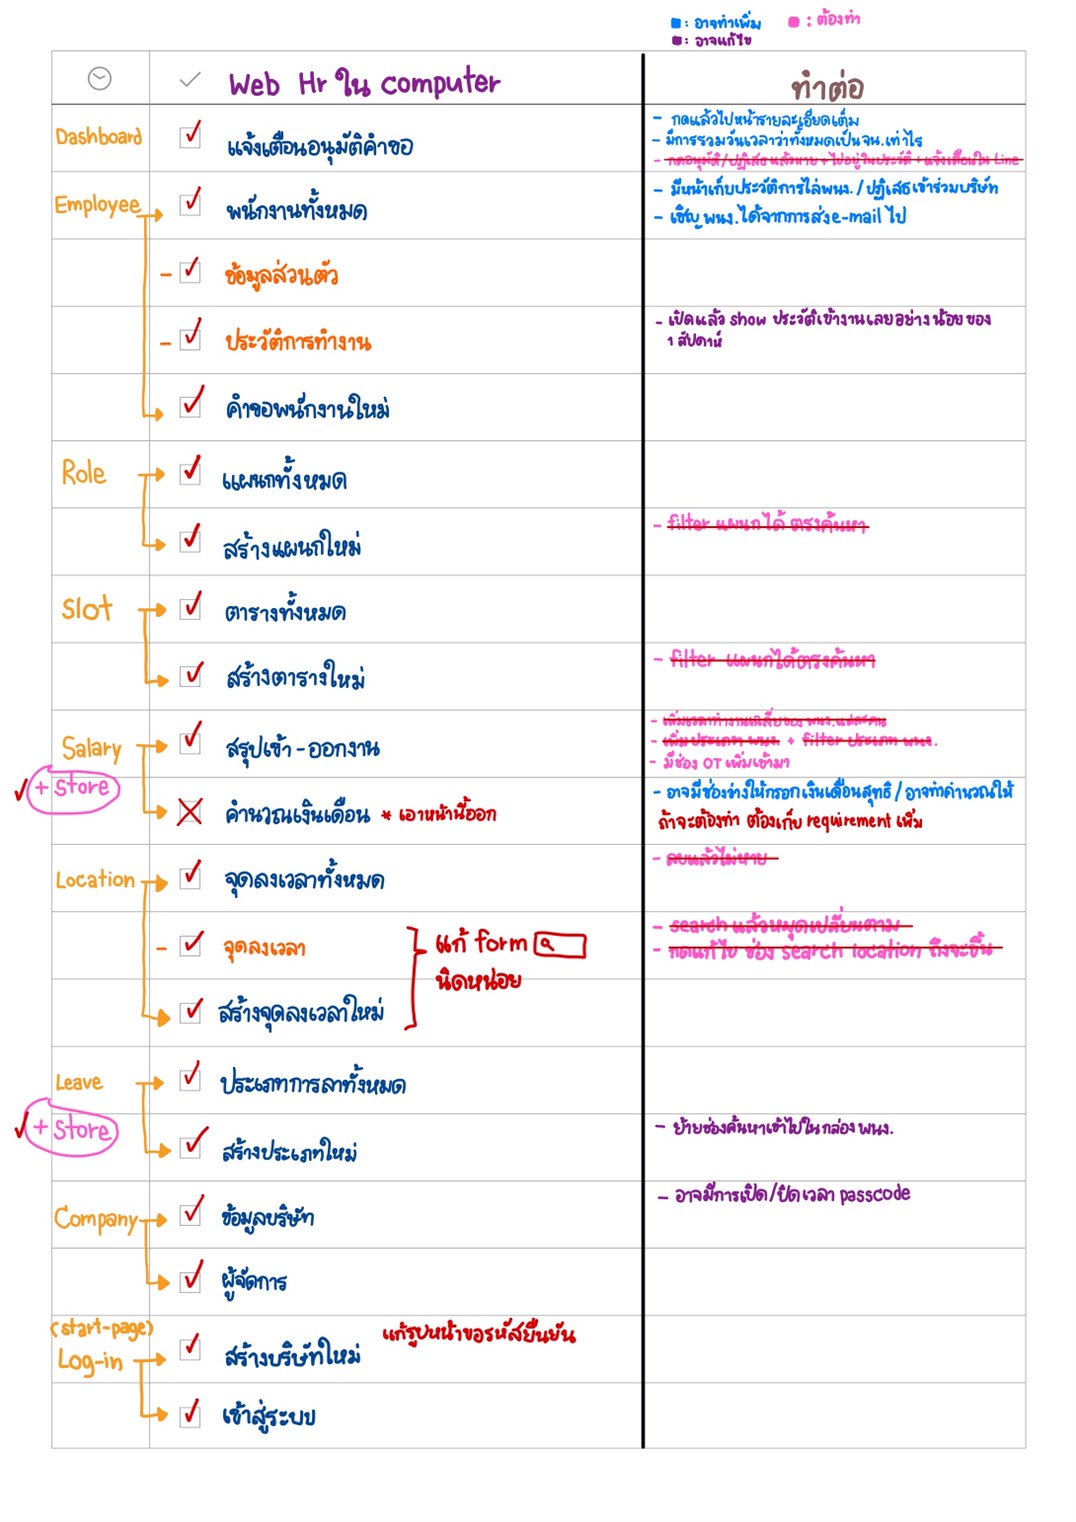
\includegraphics[width=14cm,keepaspectratio]{./images/design7.jpg}
  \end{center}
  \caption[รูปแสดงลำดับขั้นตอนการทำงานและการตรวจสอบความเรียบร้อย]{รูปแสดงลำดับขั้นตอนการทำงานและการตรวจสอบความเรียบร้อย} 
  
\end{figure}

\begin{figure}
  \begin{center}
    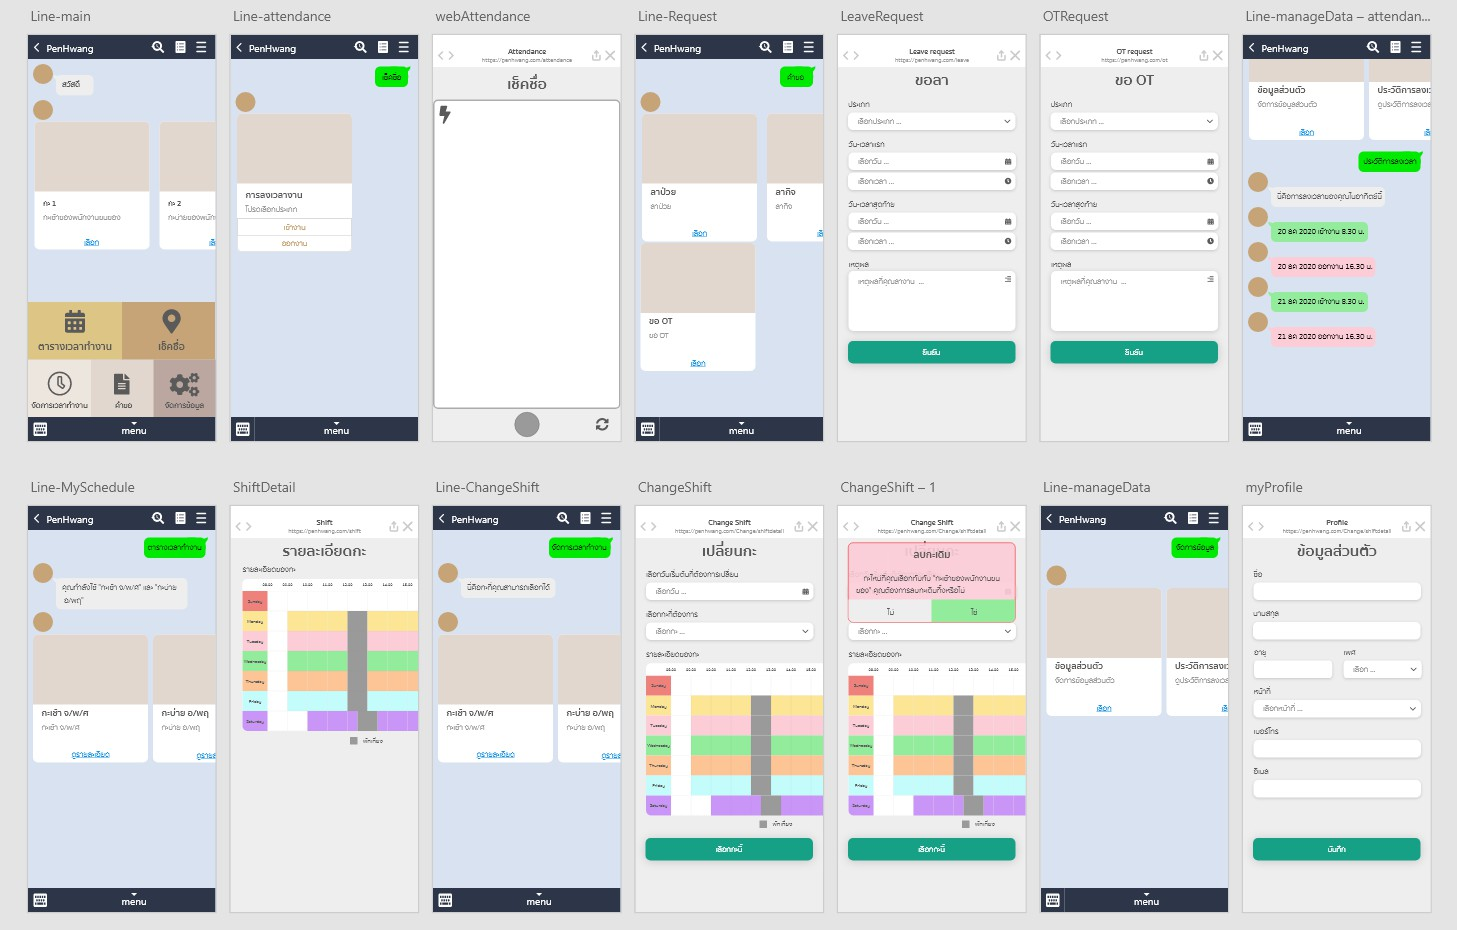
\includegraphics[width=\linewidth]{./images/design_xd.jpg}
  \end{center}
  \caption[รูปแสดงผลจากการออกแบบด้วยโปรแกรม Adobe XD]{รูปแสดงผลจากการออกแบบด้วยโปรแกรม Adobe XD} 
  
\end{figure}

\begin{figure}
  \begin{center}
    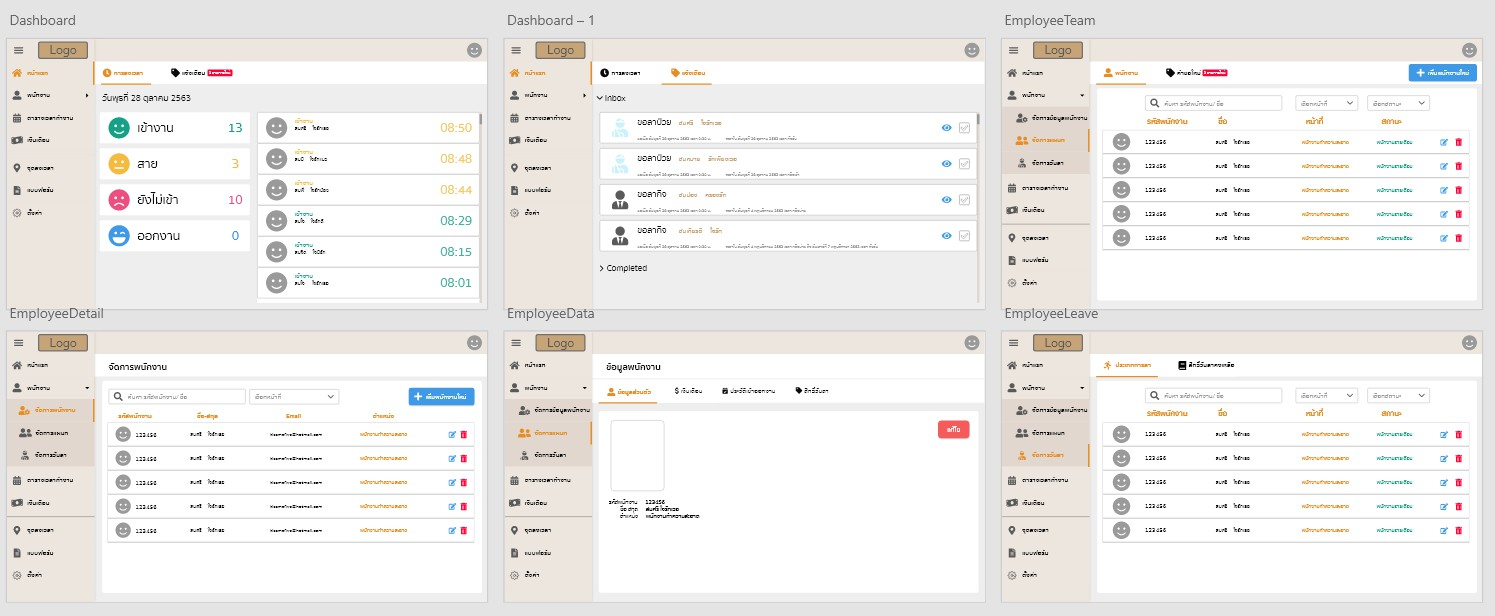
\includegraphics[width=\linewidth]{./images/design_xd2.jpg}
  \end{center}
  \caption[รูปแสดงผลจากการออกแบบด้วยโปรแกรม Adobe XD 2]{รูปแสดงผลจากการออกแบบด้วยโปรแกรม Adobe XD 2} 
  
\end{figure}
% \chapter{\ifcpe คู่มือการใช้งานระบบ\else Manual\fi}
% ฟังก์ชันที่โปรเจคนี้รองรับ และ วิธีการใช้งานมีดังนี้
% \section{สร้างบริษัทของคุณ}



% \section{code จาก GitHub}
% โปรเจคนี้ถูกแบ่งออกเป็น 3 repositories คือ 

% penhwang backend

% \url{https://github.com/TouchySarun/penhwang_backend}, 

% penhwang frontend mobile

% \url{https://github.com/Tiewly/penhwang_frontend_mobile} 

% และ penhwang frontend desktop 

% \url{https://github.com/TouchySarun/penhwang_frontend_desktop} 
% \section{โปรแกรม และ ส่วนเสริมที่จำเป็น}
% \subsection{IDE (Integrated development environment)}
% โดยโปรเจคนี้เลือกใช้ vs code เป็น IDE หาวิธี install ได้จาก \url{https://code.visualstudio.com/}
% \subsection{package manger command}
% โดยโปรเจคนี้เลือกใช้ npm เป็น package manager หาวิธี install ได้จาก npm 

% \url{https://nodejs.org/en/}
% \subsection{ส่วนเสริม}
% หลังจาก install vs code และ npm แล้ว ให้เปิด vs code ขึ้นมาและเปิด terminal โดยใช้คำสั่งลัด "ctrl + shift + p" 
% \begin{itemize}
%   \item nuxt พิมพ์คำสั่ง > npm i -g nuxt
%   \item firebase-npm เปิดไฟล์ penhwang\_backend โดย คลิกที่ File/Open Floder ... แล้วเลือกไฟล์
% จากนั้นเปิด terminal แล้ว install ส่วนเสริม โดยใช้คำสั่ง > npm i -g firebase
%   \item vue2-google-maps เปิดไฟล์ penhwang\_frontend\_desktop โดย คลิกที่ File/Open Floder ... แล้วเลือกไฟล์
% จากนั้นเปิด terminal แล้ว install ส่วนเสริม โดยใช้คำสั่ง 

% > npm i vue2-google-maps
% \end{itemize}
% \subsection{key สำหรับ API ต่าง ๆ}
% ตัวโปรเจคนี้มีความจำเป็นที่จะต้องเชื่อมต่อกับหลาย ๆ API(Application Programming Interface) เช่น firebase และ google map 
% และ แต่ละ API ต้องมี key ในการเชื่อมต่อ โดยต้องนำ key มาจากที่ต่าง ๆ ดังนี้
% \begin{itemize}
%   \item firebase โดยไปที่หน้า firebase console \url{https://console.firebase.google.com/} หากยังไม่มีโปรเจคของตนเองให้ทำการเพิ่มโปรเจคใหม่จากนั้นเข้าไปที่หน้า Project settings/general สิ่งที่ต้องการมีดังนี้
%   \begin{itemize}
%     \item apiKey
%     \item authDomain
%     \item databaseURL
%     \item projectId
%     \item storageBucket
%     \item messagingSenderId
%     \item appendixmeasurementId
%   \end{itemize}
%   นำทุกอย่างที่ต้องการใส่ในไฟล์ db.js
% \end{itemize}
% \begin{itemize}
%   \item firebase โดยไปที่หน้า firebase console \url{https://console.firebase.google.com/} หากยังไม่มีโปรเจคของตนเองให้ทำการเพิ่มโปรเจคใหม่จากนั้นเข้าไปที่หน้า Project settings/general สิ่งที่ต้องการมีดังนี้
%   \begin{itemize}
%     \item apiKey
%     \item authDomain
%     \item databaseURL
%     \item projectId
%     \item storageBucket
%     \item messagingSenderId
%     \item appendixmeasurementId
%   \end{itemize}
%   นำทุกอย่างที่ต้องการใส่ในไฟล์ db.js
% \end{itemize}

